%%%%%%%%%%%%%%%%%%%%%%%%%%%%%%%%%%%%%%%%%%%%%%%%%%%%%%%%%%%%%%%%%%%%%%
%
% レポートテンプレート
%
% updated 22 Oct, 2018
% last updated 02 Apr, 2021
%
% (c) Tohru TAKADA@UEC
% 各自のレポートに合わせて変更して使ってください.上記の行は残して使うこと.
% 2次配布可です.ご利用は計画的に.
%
%%%%%%%%%%%%%%%%%%%%%%%%%%%%%%%%%%%%%%%%%%%%%%%%%%%%%%%%%%%%%%%%%%%%%%
\documentclass[a4paper,10pt]{jarticle}
\usepackage[dvipdfmx]{graphicx}
\usepackage{amsmath}
\usepackage{latexsym}
\usepackage{multirow}
\usepackage{url}
\usepackage{float}
\setlength{\textwidth}{165mm} %165mm-marginparwidth
\setlength{\marginparwidth}{40mm}
\setlength{\textheight}{225mm}
\setlength{\topmargin}{-5mm}
\setlength{\oddsidemargin}{-3.5mm}

\def\vector#1{\mbox{\boldmath $#1$}}
\newcommand{\AmSLaTeX}{%
 $\mathcal A$\lower.4ex\hbox{$\!\mathcal M\!$}$\mathcal S$-\LaTeX}
\newcommand{\PS}{{\scshape Post\-Script}}
\def\BibTeX{{\rmfamily B\kern-.05em{\scshape i\kern-.025em b}\kern-.08em
 T\kern-.1667em\lower.7ex\hbox{E}\kern-.125em X}}
\newcommand{\pderiv}[2]{{\partial#1\over\partial#2}}
\newcommand{\deriv}[2]{{{\rm d}#1\over{\rm d}#2}}
\newcommand{\dderiv}[2]{{{\rm d}^2#1\over{\rm d}#2^2}}
\newcommand{\DeLta}{{\mit\Delta}}
\renewcommand{\d}{{\rm d}}
\def\wcaption#1{\caption[]{\parbox[t]{100mm}{#1}}}
\def\rm#1{\mathrm{#1}}
\def\tempC{^\circ \rm{C}}

\makeatletter
%\def\section{\@startsection {section}{1}{\z@}{-3.5ex plus -1ex minus % -.2ex}{2.3ex plus .2ex}{\Large\bf}}
\def\section{\@startsection {section}{1}{\z@}{-3.5ex plus -1ex minus
-.2ex}{2.3ex plus .2ex}{\normalsize\bf}}
\makeatother

\makeatletter
\def\subsection{\@startsection {subsection}{1}{\z@}{-3.5ex plus -1ex minus
-.2ex}{2.3ex plus .2ex}{\normalsize\bf}}
\makeatother

\makeatletter
\def\@seccntformat#1{\@ifundefined{#1@cntformat}%
   {\csname the#1\endcsname\quad}%      default
   {\csname #1@cntformat\endcsname}%    enable individual control
}
\makeatother

%%%%%%%%%%%%%%%%%%%%%%%%%%%%%%%%%%%%%%%%%%%%%%%%%%%%%%%%%%%%%%%%%%%%%%
\begin{document}

%
%% 通常は指定の表紙を付けて印刷して提出していますが,電子データをアップロードする際は
%% 表紙は付けなくても結構です.冒頭にタイトル,所属,学籍番号,氏名と記載日
%% 修正版を提出する際は更新日を書いてください
%
\begin{center}
{\Large{\bf K演習第6回レポート課題}} \\
{\bf Aクラス 2311009 アハメドアティフ} \\

\end{center}
%%%%%%%%%%%%%%%%%%%%%%%%%%%%%%%%%%%%%%%%%%%%%%%%%%%%%%%%%%%%%%%%%%%%%%
\section{宿題1}

\begin{enumerate}
	\setlength{\itemsep}{-2mm}
	 \item 問題文より,ある病気の感染率は0.5%であるから,その周辺確率は0.005で,感染していない確率は感染している場合の補集合より,0.995.よって,病気の感染の有無に関する周辺確率表は以下のようになった.
	 
	 \begin{table}[ht]
		\begin{center}
		% \caption{タイトル}
		\label{tab1}
		\begin{tabular}{lll}\hline
		感染 & あり & なし\\ \hline
		周辺確率 & 0.005 & 0.995\\ \hline
		\end{tabular}
		\end{center}
		\end{table}


	 \item 問題文より,感染している時に診断結果でも「あり」と診断される確率は0.80より,診断結果で「なし」と判定される確率は0.20.また,感染していない時に「あり」という診断結果が出る確率は0.10であるから,「なし」という診断結果が出るのは0.90.
	 したがって,患者の感染の有無が判明しているときのそれぞれの診断結果の条件付確率表は以下のようになった.
	
	 \begin{table}[ht]
		\begin{center}
		\label{tab2}
		\begin{tabular}{|c|cc|}\hline
    {} & \multicolumn{2}{c|}{診断結果} \\
		 & あり & なし \\ \hline
    感染あり & 0.80 & 0.20 \\
		感染なし & 0.10 & 0.90 \\ \hline
		\end{tabular}
		\end{center}
		\end{table}

	 \item 「診断結果が感染ありであった」という結果を得た患者が実際に感染している確率は,ベイズの定理から,式\ref*{equ1}のようになった.
	 
	 \begin{equation}
		\label{equ1}
		\frac{0.80 \times 0.005}{0.80 \times 0.005 \times 0.10 \times 0.095}=\frac{8}{207}\approx  0.0386
	 \end{equation}

	 上記の式より\fbox{0.0386}が求めたい確率である.

	 \vspace{3mm}

	 \item 診断方法Bの時の,「診断結果が感染ありだった」時に患者が実際の感染している確率は,ベイズの定理より,以下の式\ref*{equ2}のようになった
	 
	 \begin{equation}
		\label{equ2}
		\begin{split}
			P(有|あり) &= \frac{P(あり|有)P(有)}{P(あり|有)P(有)+P(あり|無)P(無)} \\
			&= \frac{0.90 \times 0.005}{0.90 \times 0.005 \times 0.20 \times 0.995} \\
			&= \frac{9}{407} \approx 0.0221
		\end{split}
	 \end{equation}
	 
	 したがって,求めたい確率は\fbox{0.0221}である.

	\end{enumerate}

%%%%%%%%%%%%%%%%%%%%%%%%%%%%%%%%%%%%%%%%%%%%%%%%%%%%%%%%%%%%%%%%%%%%%%
\section{宿題2}

\begin{enumerate}
	\setlength{\itemsep}{-2mm}
	 \item (a)累積分布関数$F(x)$を描いたグラフは図\ref*{apara}の通りである.
	 
	 \vspace{3mm}

	 \begin{figure}[ht]
		\begin{center}
		 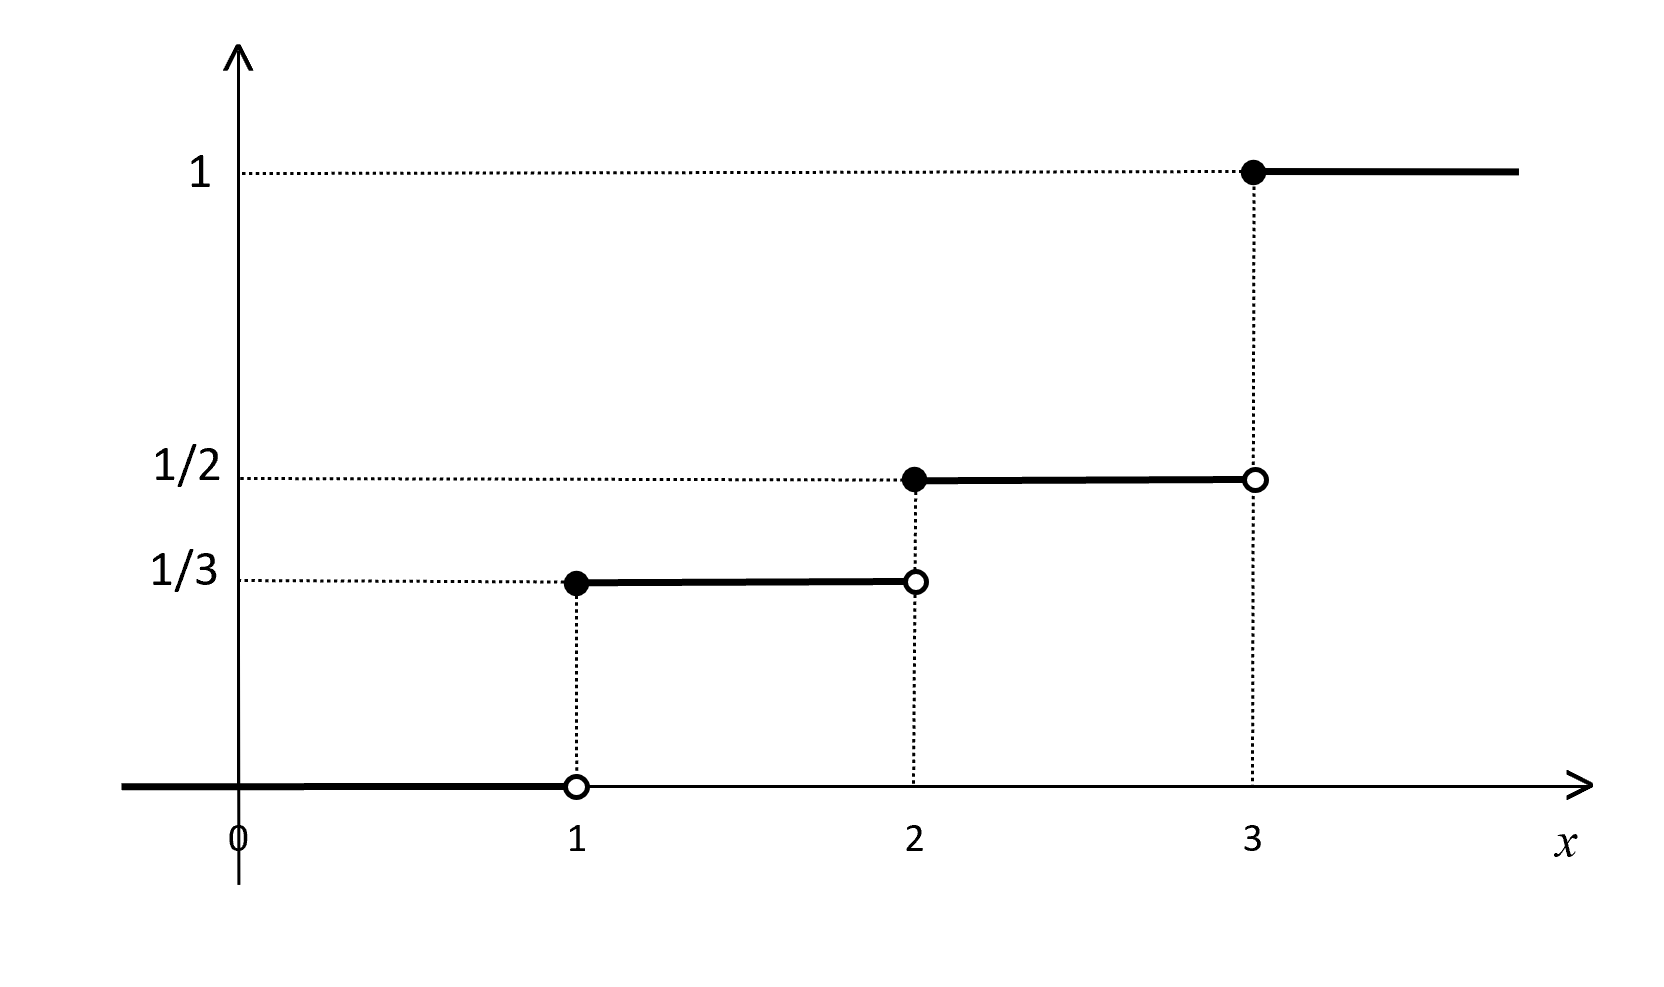
\includegraphics[scale=1.0]{zu4.png}
		 \caption{宿題2-1の累積分布関数}
		 %\ecaption{Options of documentclass.}
		 \label{apara}
		\end{center}
		\end{figure}

				(b)$X$の平均と分散は以下の式\ref*{equ3}と式\ref*{equ4}のように求められた.

	\begin{equation}
		\label{equ3}
		\begin{split}
			E[X] &= \sum_{k = 1}^{3}x_{k} p_{k} = 1 \times \frac{1}{3} + 2 \times \frac{1}{6} + 3 \times \frac{1}{2} = \frac{13}{6}
		\end{split}
	\end{equation}

	\begin{equation}
		\label{equ4}
		\begin{split}
			V[X] &= E[X^2]-{E[X]}^2 \\
					 &= 1^2 \times \frac{1}{3} +2^2 \times \frac{1}{6} +3^2 \times \frac{1}{2} - \frac{13^2}{6^2} \\
					 &= \frac{1}{3}+\frac{2}{3}+\frac{9}{2}-\frac{169}{36} \\
					 &= \frac{29}{36}
		\end{split}
	\end{equation}

	よって,平均は\fbox{$\frac{13}{6}$},分散は\fbox{$\frac{29}{36}$}である.
		\vspace{3mm}

	 \item 確率変数Xが一回に1.5の費用がかかる回収額を表すときのこの投資のリターンの平均と標準偏差は,線形性から,以下の式と式のように求められた.

	 \begin{equation}
		\label{equ5}
		E[X-1.5] = E[X] - 1.5 = \frac{13}{6} - \frac{3}{2} = \frac{2}{3}
	 \end{equation}
	 
	 \begin{equation}
		\label{equ6}
		\sigma[X-1.5] = \sqrt{V[X-1.5]} = \sqrt{V[X]} = \frac{\sqrt{29}}{6}
	 \end{equation}

	 したがって,求める平均は\fbox{$\frac{2}{3}$},標準偏差は\fbox{$\frac{\sqrt{29}}{6}$}である.

	 \vspace{3mm}

	 \item (a)与式の確率変数$X$の確率密度関数$f(x)$の累積分布関数は以下の図\ref*{apara2}のように描けた.
	 
	 \begin{figure}[H]
		\begin{center}
		 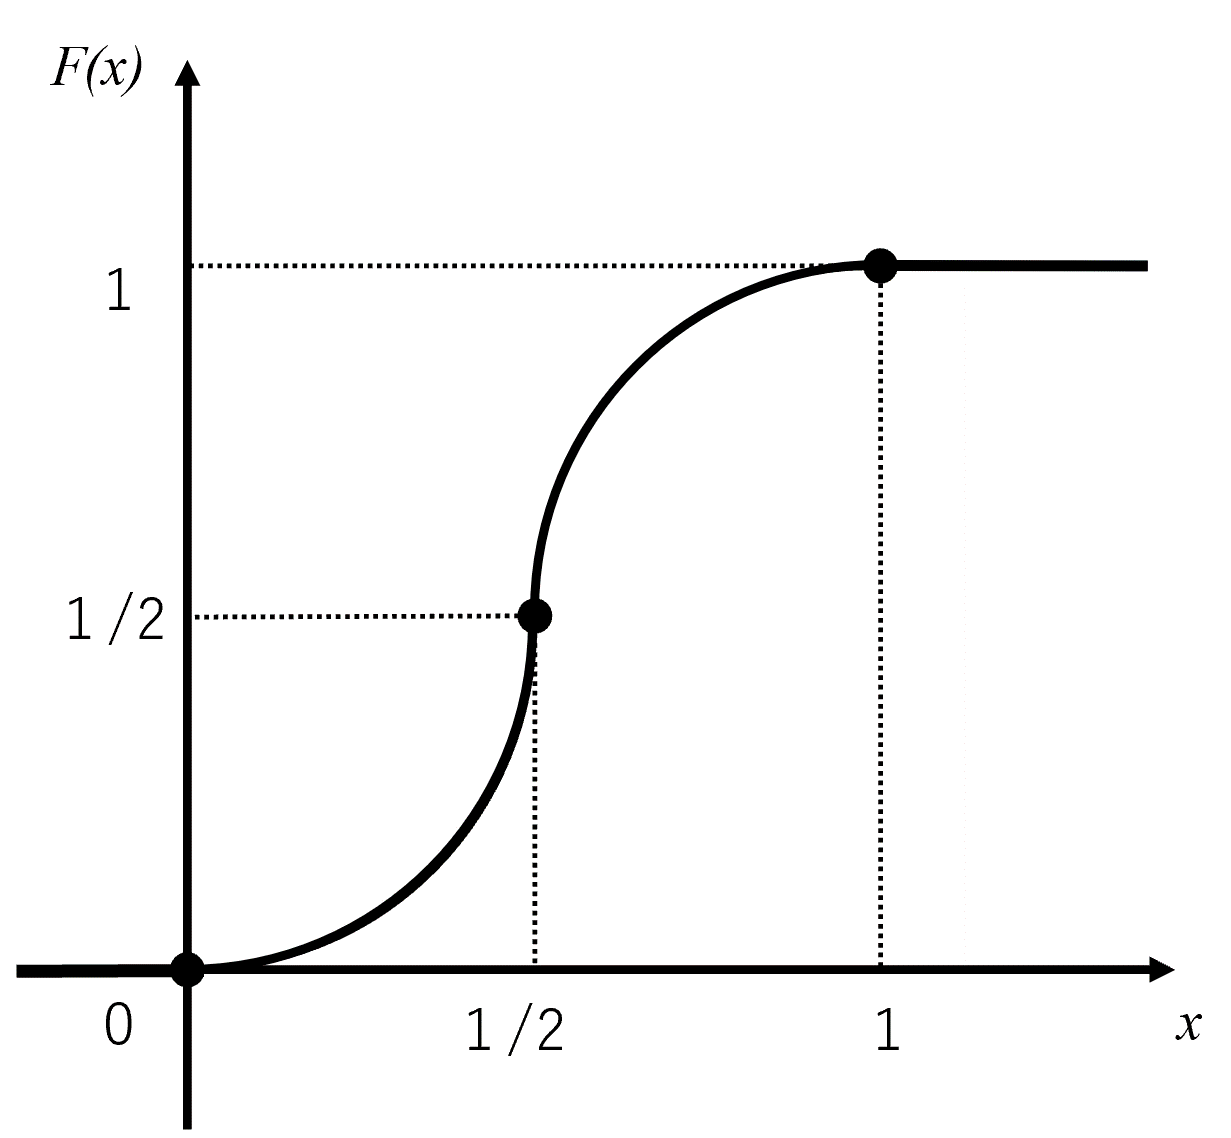
\includegraphics[scale=1.0]{zu5.png}
		 \caption{宿題2-3の累積分布関数}
		 %\ecaption{Options of documentclass.}
		 \label{apara2}
		\end{center}
		\end{figure}

		(b)次に$X$の平均と分散は以下の式\ref*{equ7},式\ref*{equ8},式\ref*{equ9}のように求められた.

		\begin{equation}
			\label{equ7}
			\begin{split}
				E[X] &= \int_{0}^{1} xf(x) \,dx \\
						 &= \int_{0}^{\frac{1}{2}} x(4x) \,dx + \int_{\frac{1}{2}}^{1} x(-4x+4) \,dx \\
						 &= \frac{4}{3}[x^3]_{0}^{\frac{1}{2}}+ [-\frac{4}{3}x^3+2x^2]_{\frac{1}{2}}^{1} \\
						 &= \frac{1}{6}+\frac{2}{3}-\frac{1}{3} \\
						 &= \frac{1}{2}
			\end{split}
		\end{equation}

		\begin{equation}
			\label{equ8}
			\begin{split}
				E[X^2] &= \int_{0}^{1} x^2 f(x) \,dx \\
							 &= \int_{0}^{\frac{1}{2}} x^2(4x) \,dx + \int_{\frac{1}{2}}^{1} x^2(-4x+4) \,dx \\
							 &= [x^4]_{0}^{\frac{1}{2}} + [-x^4+\frac{4}{3}x^3]_{\frac{1}{2}}^{1} \\
							 &= \frac{1}{16}+\frac{1}{3}-\frac{5}{48} \\
							 &= \frac{7}{24} \\
							\end{split}
		\end{equation}

		\begin{equation}
			\label{equ9}
				V[X] = E[X^2]- {E[X]}^2 = \frac{7}{24}-{\frac{1}{2}}^2 =\frac{1}{24} \\
		\end{equation}

よって,平均は\fbox{$\frac{1}{2}$},分散は\fbox{$\frac{1}{24}$}である.

	\end{enumerate}
	\vspace{3mm}
%%%%%%%%%%%%%%%%%%%%%%%%%%%%%%%%%%%%%%%%%%%%%%%%%%%%%%%%%%%%%%%%%%%%%%
\section{宿題3-1}
与えられた確率表とその期待値$\mu$と分散$\sigma^2$から,任意の実数$a$を用いて,分散$\sigma^2$は以下の式\ref*{equa}のように変形できる.

\begin{equation}
	\label{equa}
	\begin{split}
		\sigma^2 &= E[(X-\mu)^2] \\
						 &= \sum_{k=1}^{N} (k-\mu)^2 p_k \\
						 &\geq \sum_{k:(k-\mu)\leq -a} (k-\mu)^2 p_k + \sum_{k:(k-\mu)\geq a} (k-\mu)^2 p_k \\
						 &\geq \sum_{k:(k-\mu)\leq -a} a^2 p_k + \sum_{k:(k-\mu)\geq a} a^2 p_k \\
						 &\geq a^2 \left\{  \sum_{k:(k-\mu)\leq -a} p_k + \sum_{k:(k-\mu)\geq a} p_k \right\} \\
						 &= a^2 P\left((X-\mu)^2\geq a^2\right) 
	\end{split}
\end{equation}

よって,式\ref*{equa}の両辺を$a^2$で割って,対称性から$a>0$の任意の実数$a$を考えてあげることによって,以下のチェビチェフの不等式が証明された.

\begin{equation}
	\label{equa}
		\frac{\sigma^2}{a^2} = P\left(|X-\mu|\geq a\right)
\end{equation}

\vspace{3mm}
%%%%%%%%%%%%%%%%%%%%%%%%%%%%%%%%%%%%%%%%%%%%%%%%%%%%%%%%%%%%%%%%%%%%%%
\section{宿題3-2}

\begin{enumerate}
	\item マルコフの不等式から
	\begin{equation}
		P(X\geq800)\leq\frac{400}{800}=\frac{1}{2}
	\end{equation}

	よって,求める最大の割合は\fbox{$\frac{1}{2}$}である.

	\item マルコフの不等式から
	\begin{equation}
		P(X\geq10000)\leq\frac{20}{10000}=\frac{1}{500}
	\end{equation}

	よって,求める最大の割合は\fbox{$\frac{1}{500}$}である.

	\item チェビチェフの不等式から
	\begin{equation}
		P(X-400\geq800-400)\leq P(|X-400|\geq400)\leq\frac{200^2}{400^2}=\frac{1}{4}
	\end{equation}

	よって,求める最大の割合は\fbox{$\frac{1}{4}$}である.

	\item チェビチェフの不等式から
	\begin{equation}
		P(X-400\geq10000-400)\leq P(|X-400|\geq9600)\leq\frac{200^2}{9600^2}=\frac{1}{2304}
	\end{equation}

	よって,求める最大の割合は\fbox{$\frac{1}{2304}$}である.
\end{enumerate}

%%%%%%%%%%%%%%%%%%%%%%%%%%%%%%%%%%%%%%%%%%%%%%%%%%%%%%%%%%%%%%%%%%%%%%
\end{document}

\begin{figure}[ht]
\begin{center}
 \includegraphics[scale=0.5]{ファイル名}
 \caption{タイトル}
 %\ecaption{Options of documentclass.}
 \label{apara}
\end{center}
\end{figure}

\begin{table}[ht]
\begin{center}
\caption{タイトル}
\label{tab1}
\begin{tabular}{ll}\hline
col1 & col2 \\ \hline
val1 & val2 \\
val3 & val4 \\ \hline
\end{tabular}%
\end{center}
\end{table}

%箇条書き
\begin{itemize}
	\setlength{\itemsep}{-2mm}
	 \item 測定上特に注意をした点(注意をしなければならなかった点)
	 \item 測定装置で特に説明をしなければ何故,どのように測定値を取得したのか
			 読者にわからない点
	 \item 実験結果を再現するために必要な特別な手順や測定方法など
	 \item 測定データを処理する際に利用したソフトウェアで特に記載が必要なもの
	\end{itemize}
	
	%番号振って箇条書き
	\begin{enumerate}
	\setlength{\itemsep}{-2mm}
	 \item 電圧はディジタルマルチメーターを用いて測った
	 \item まずディジタルマルチメーターの電源をONにした
	 \item 次にメーターのプローブを電源端子に接続し$\cdots$
	\end{enumerate}